\section{Exercises}

%%%%%%%%%%%%%%%%%%%%%%%%%%%%%%%%%%%%%

\subsection{Defining probability}

%%%%%%%%%%%%%%%%%%%%%%%%%%%%%%%%%%%%%

% LLN

\eoce{True or false: If a fair coin is tossed many times and the last eight tosses are all heads, then the chance that the next toss will be heads is somewhat less than 50\%.}
{False. Since these are independent trials the probability does not change from trial to trial and does not depend on what the outcome was on the previous trial(s). Therefore, in the next toss the probability of getting a head will still be 0.5.}


\eoce{Determine if the below statements are true of false and explain your reasoning.
\begin{enumerate}[(a)]
\setlength{\itemsep}{0mm}
\item Drawing a face card (jack, queen, or king) and drawing a red card from a full deck of playing cards are mutually exclusive events.
\item Drawing a face card and drawing an ace from a full deck of playing cards are mutually exclusive events.
\end{enumerate}
}
{
\begin{enumerate}[(a)]
\item False. There are red face cards (jack, queen, or king of hearts and diamonds). Since a card can be both a face card and a red card, the two events are not mutually exclusive.
\item True. A card cannot be both a face card and an ace.
\end{enumerate}
}


\eoce{Below are four scenarios, each describing two games. In the first game, a coin is tossed 10 times. In the second game, a coin is tossed 100 times. For each scenario, if you could only play one game, which would you play? Explain your reasoning.
\begin{enumerate}[(a)]
\setlength{\itemsep}{0mm}
\item If it is heads more than 60\% of the time, you win \$1.
\item If it is heads more than 40\% of the time, you win \$1.
\item If it is heads between 40\% and 60\% of the time, you win \$1.
\item If it is heads less than 30\% of the time, you win \$1.
\end{enumerate}
} 
{
\begin{enumerate}[(a)]
\item 10 tosses. Since the desired outcome is larger than the expected proportion of heads (50\%), we would want fewer trials (flips). With a low number of flips the variability in the number of heads observed is much larger. For example, we wouldn't be very surprised if 7 out of 10 flips were heads. On the other hand, with 100 flips, we would be surprised if 70 out of 100 flips were heads. With 100 flips it would be more likely to get 50\% heads and 50\% tails, which is not what we want.
\item 100 tosses. The expected proportion of 50\% is greater than 40\% and with more flips the observed proportion of heads would be closer to the expected value.
\item 100 tosses. The expected proportion of 50\% is between 40\% and 60\%. With more flips the observed proportion of heads would be closer to the expected value.
\item 10 tosses. The desired proportion of heads (less than 30\%) is below the expected proportion and with fewer flips it would be more likely to observe a proportion that is not close to the expected value.
\end{enumerate}
}

% Probabilities (dice) - Independence (2.1.5)

\eoce{Backgammon is a board game for two players in which the playing pieces are moved according to the roll of two dice. Players win by removing all of their pieces from the board therefore it is good to roll high numbers. You are playing backgammon with a friend and you roll two double sixes in a row while your friend rolled first double ones and then double threes. Double sixes means that in a single roll of two dice, each die comes up as a six. Double threes means each die comes up as a three, etc. Your friend claims that you are cheating because it is very unlikely to be able to roll two double sixes in a row. Using probabilities how could you argue that your rolls were just as likely as his?
% in the second sentence, it's not clear that moving pieces corresponds to removing them and then winning.  how about redoing the second sentence: "Players win by moving their pieces all of the way across the board, therefore..."
}
{
\begin{align*}
P(\text{your rolls}) &= P(\text{six and six on the first roll and six and six on the second roll}) \\ 
&= P(\text{six and six on the first roll}) * P(\text{six and six on the second roll}) \\
&= (1/6 * 1/6) * (1/6 * 1/6) = 0.00077 \\
P(\text{friend's rolls}) &= P(\text{one and one on the first roll and three and three on the second roll}) \\
&= P(\text{one and one on the first roll}) * P(\text{three and three on the second roll}) \\ 
&= (1/6 * 1/6) * (1/6 * 1/6) = 0.00077
\end{align*}
Both outcomes have equal probability, therefore it is just as likely to roll two double sixes in a row as rolling first double ones and then double threes.
}

% Probabilities (coin) - Independence (2.1.5)

\eoce{If you flip a fair coin 10 times, what is the probability of
\begin{multicols}{3}
\begin{enumerate}[(a)]
\setlength{\itemsep}{0mm}
\item getting all tails? 
\item getting all heads? 
\item getting at least one tail? 
\end{enumerate}
\end{multicols}
}
{
\begin{enumerate}[(a)]
\item P(all tails) = $0.5^{10}$ = 0.00098.
\item P(all heads) = $0.5^{10}$ = 0.00098.
\item P(at least one tail) = 1 - P(no tails) = 1 - (0.5$^{10}$) = 1 - 0.001 = 0.999.
\end{enumerate}
}

% Probabilities (dice) - Independence

\eoce{If you roll a two fair dice, what is the probability of
\begin{multicols}{3}
\begin{enumerate}[(a)]
\setlength{\itemsep}{0mm}
\item getting a sum of 1?
\item getting a sum of 5?
\item getting a sum of 12?
\end{enumerate}
\end{multicols}
}
{
\begin{enumerate}[(a)]
\item P(sum of 1) = 0. Since there are two dice being rolled, the minimum possible sum is 2.
\item P(sum of 5) = P(1,4) +  P(4,1) + P(2,3) + P(3,2) = $\left( \frac{1}{6} * \frac{1}{6} \right)$ * 4 = $\frac{4}{36}$ =  0.11.
\item P(sum of 12) = P(6,6) = $\left( \frac{1}{6} * \frac{1}{6} \right)$ = $\frac{1}{36}$.
\end{enumerate}
}

% Venn diagrams

\eoce{An online survey shows that 25\% of bloggers own a DSLR camera, 90\% own a point-and-shoot camera, and 20\% own both types of cameras.
\begin{enumerate}[(a)]
\setlength{\itemsep}{0mm}
\item Draw a Venn diagram summarizing these probabilities.
\item What percent of bloggers own a DSLR but not a point-and-shoot camera?
\item What percent of bloggers own a point-and-shoot camera but not a DSLR?
\item What percent of bloggers own either a point-and-shoot camera or a DSLR?
\item What percent of bloggers own neither a DSLR nor a point-and-shoot camera?
\item Are owning a DSLR and point-and-shoot camera mutually exclusive?
\end{enumerate}
}
{
\begin{enumerate}[(a)]
\item The Venn diagram is shown below:
\begin{center}
\includegraphics[width=70mm]{02/figures/eoce/psDslrVenn.png}
\end{center}
\item P(DSLR but not point\&shoot) = P(DSLR) - P(DSLR and point\&shoot) = 0.25 - 0.20 = 0.05.
\item P(point\&shoot but not DSLR) = P(point\&shoot) - P(DSLR and point\&shoot) = 0.90 - 0.20 = 0.70.
\item P(DSLR or point\&shoot) = P(DSLR) + P(point\&shoot) - P(DSLR and point\&shoot) = 0.25 + 0.90 - 0.20 = 0.95.
\item P(neither DSLR nor point\&shoot) = 1 - P(DSLR or point\&shoot)  = 1 - 0.95 = 0.05.
\item No, there are bloggers who own both types of cameras.
\end{enumerate}
}\label{cameras}

%

\eoce{In a class where everyone's native language is English, 70\% of students speak Spanish, 45\% speak French as a second language and 20\% speak both.  Assume that there are no students who speak  another second language. 
\begin{enumerate}[(a)]
\setlength{\itemsep}{0mm}
\item Draw a Venn diagram summarizing these probabilities.
\item What percent of students speak Spanish but not French?
\item What percent of students speak French but not Spanish?
\item What percent of students speak some second language?
\item What percent of the students do not speak a second language? 
\item Are speaking French and Spanish mutually exclusive?
\end{enumerate}
}
{
\begin{enumerate}[(a)]
\item The Venn diagram is shown below:
\begin{center}
\includegraphics[width=70mm]{02/figures/eoce/SpanishFrenchVenn.png}
\end{center}
\item P(Spanish but not French) = P(Spanish) - P(Spanish and French) = 0.70 - 0.20 = 0.50.
\item P(French but not Spanish) = P(French) - P(Spanish and French) = 0.45 - 0.20 = 0.25.
\item P(Spanish or French) = P(Spanish) + P(French) - P(Spanish and French) = 0.70 + 0.45 - 0.20 = 0.95.
\item P(neither Spanish nor French) = 1 - P(Spanish or French)  = 1 - 0.95 = 0.05.
\item No, there are students who speak both languages; P(Spanish and French) $\ne$ 0.
\end{enumerate}
}\label{languages}

%

\eoce{The below exercises are designed to help you understand the how the concepts of independence and mutual exclusivity relate to each other.
\begin{enumerate}[(a)]
\setlength{\itemsep}{0mm}
\item Is it possible that both you and a randomly selected student from your class earn an A in this course? Are these two events mutually exclusive? Are they independent?
\item Is it possible that both you and a friend you study with from your class earn an A in this course? Are these two events mutually exclusive? Are they independent?
\item If two events can occur at the same time must they be dependent?
\end{enumerate}
}
{
\begin{enumerate}[(a)]
\item Yes, it is possible that both you and a randomly selected student from your class gets an A in this course, therefore these two events are not mutually exclusive. They are probably independent though since how well you do in the course is not dependent on how well a randomly selected student does.
\item Yes, it is possible that both you and a friend you study with from your class gets an A in this course, therefore these two events are not mutually exclusive. They are also probably not independent: if you study together how well one of you do in the course might depend on the other.
\item No, in part (a) we described two events that can occur at the same time but are not dependent.
\end{enumerate}
}

% Probabilities (independent)

\eoce{In a multiple choice exam there are 5 questions and 4 choices for each question (a, b, c, d). Nancy has not studied for the exam at all, and decided to randomly guess the answers. What is the probability that:
\begin{enumerate}[(a)]
\setlength{\itemsep}{0mm}
\item The first question she gets right is the $5^{th}$ question?
\item She gets all questions right?
\item She gets at least one question right?
\end{enumerate}
}
{
\begin{enumerate}[(a)]
\item Since she is randomly guessing, probability of getting each question right is $p = 0.25$. Then, \\
P(\underline{Wrong} \underline{Wrong} \underline{Wrong} \underline{Wrong} \underline{Right}) = $0.75^4 * 0.25 = 0.07910156 \approx 0.0791$.
\item P(\underline{Right} \underline{Right} \underline{Right} \underline{Right} \underline{Right}) = $0.25^5 = 0.0009765625 \approx 0.0010$.
\item P(at least 1 Right) = 1 - P(none Right) = $1 - 0.75^5 = 1 - 0.2373 = 0.7627$.
\end{enumerate}
}

% Probabilities (independent)

\eoce{The US Census is conducted every 10 years and collects demographic information from the residents of United States. The table below shows the distribution of the level highest education obtained by US residents by gender. Answer the following questions based on this table.
\begin{center}
\begin{tabular}{l p{5cm} c c }
&						& \multicolumn{2}{c}{\textit{Gender}} \\
\cline{3-4}
&								& Male	& Female \\
\cline{2-4}
& Less than high school				&0.19	&0.19	 \\
& High school graduate 				&0.28	&0.30	 \\
\textit{Highest} & Some college			&0.27	&0.28	 \\
\textit{education} & Bachelor's degree	&0.16	&0.15	 \\ 
\textit{attained} & Master's degree		&0.06	&0.06	 \\
& Professional school degree			&0.03	&0.01	 \\
& Doctorate degree					&0.01	&0.01	 \\
\cline{2-4}
\end{tabular}
\end{center}
\begin{enumerate}[(a)]
\setlength{\itemsep}{0mm}
\item What is the probability that a randomly chosen man has at least a Bachelor's degree?
\item What is the probability that a randomly chosen woman has at least a Bachelor's degree?
\item What is the probability that a man and a woman getting married both have at least a Bachelor's degree?
\item What assumption did you make to calculate the probability in part (d)? Do you think this assumption is reasonable? 
\end{enumerate}
}
{
\begin{enumerate}[(a)]
\item P(at least a Bachelor's degree $|$ male) = 0.16 + 0.06 + 0.03 + 0.01 = 0.26
\item P(at least a Bachelor's degree $|$ female) = 0.15 + 0.06 + 0.01 + 0.01 = 0.23
\item P(man and woman both have at least a Bachelor's degree) = 0.26 * 0.23 = 0.0598
\item We assumed that the education level of the husband and wife are independent. This may not be an unreasonable assumption since people often marry people who have a comparable level of education to theirs.
\end{enumerate}
}

% Probabilities (independent)

\eoce{A middle school estimates that 20\% of its students miss one day of school per semester due to sickness, 13\% miss two days, and 5\% miss three or more days. 
\begin{enumerate}[(a)]
\setlength{\itemsep}{0mm}
\item What is the probability that a student chosen at random
\begin{enumerate}[i.]
\setlength{\itemsep}{0mm}
\item doesn't miss any days of school due to sickness?
\item misses no more than one day?
\item misses at least one day?
\end{enumerate}
\item If a parent has two kids at this middle school, can you calculate the probability that neither will miss any school as $(P(no~miss))^2$ where $P(no~miss)$ is the probability you calculated earlier? Explain.
\item Regardless of your answer to part (b) calculate the following probabilities for a parent who has two kids at this middle school.
\begin{enumerate}[i.]
\setlength{\itemsep}{0mm}
\item Neither kid will miss any school.
\item Both kids will miss some school, i.e. at least one day.
\item At least one kid will miss some school.
\end{enumerate}
\end{enumerate}
}
{
\begin{enumerate}[(a)]
\item
\begin{enumerate}[i.]
\item P(no misses) = 1 - (0.20 + 0.13 + 0.05) = 0.62
\item P(at most 1 miss) = P(no misses) + P(1 miss) = 0.62 + 0.20 = 0.82
\item P(at least 1 miss) = P(1 miss) + P(2 misses) + P(3+ misses) = 1 - P(no misses) \\
= 1 - 0.62 = 0.38
\end{enumerate}
\item No, this calculation assumes that whether or not one kid misses school should be independent of the other. These kids are siblings and if one gets sick chances are the other one will get sick as well. So whether or not one misses school due to sickness is probably not independent of the other.
\item 
\begin{enumerate}[i.]
\item P(neither miss any) = P(no miss) * P(no miss) = $0.62^2$ = 0.3844
\item P(both miss some) = P(at least 1 miss) * P(at least 1 miss) = $0.38^2$ = 0.1444
\item P(at least 1 misses some school)  = P(one misses some) + P(both miss some) \\
= 2(0.62 * 0.38) + 0.1444 = 0.6156
\end{enumerate}
\end{enumerate}
}\label{middleSchoolSick}

% Discrete probability distributions

\eoce{Indicate what, if anything, is wrong with the following probability distributions for grade breakdown in a Statistics class.
\begin{center}
\begin{tabular}{l  ccccc} 
	& \multicolumn{5}{c}{\textit{Grades}} \\
\cline{2-6}
	& A		& B 		& C 		& D		& F  \\
\cline{2-6}
(a) 	& 0.3 	& 0.3 	& 0.3 	& 0.2 	& 0.1\\
(b) 	& 0	 	& 0	 	& 1		& 0		& 0 \\
(c) 	& 0.3 	& 0.3 	& 0.3		& 0.1		& 0 \\
(d) 	& 0.3 	& 0.5 	& 0.2		& 0.1		& -0.1 \\
(e) 	& 0.2 	& 0.4 	& 0.2		& 0.1		& 0.1 \\
(f) 	& 0	 	& -0.1 	& 1.1		& 0		& 0 \\
\end{tabular}
\end{center}
}
{
\begin{enumerate}[(a)]
\item This probability distribution is wrong because sum of probabilities for all possible outcomes cannot be greater than 1 (0.3 + 0.3 + 0.3 + 0.2 + 0.1 = 1.2).
\item This probability distribution is right because sum of probabilities add up to 1, and probabilities can equal 0. The distribution shows that the entire class got C's.
\item This probability distribution is wrong because sum of probabilities for all possible outcomes cannot be smaller than 1 (0.3 + 0.3 + 0.3 + 0.1 + 0 = 0.9).
\item This probability distribution is wrong because probabilities cannot be negative, even if the sum of all possible outcomes add up to 1.
\item This probability distribution is right because sum of the probabilities add up to 1 and there are no negative probabilities (0.2 + 0.4 + 0.2 + 0.1 + 0.1 = 1).
\item This probability distribution is wrong because probabilities cannot be greater than 1 or negative, even if the sum of all possible outcomes add up to 1.
\end{enumerate}
}

% Probabilities (contingency table)

\eoce{The table below shows the relationship between hair color and eye color for a group of 1,770 German men. You might recognize this table from Chapter 1 exercises. Here we will take another look at it from a probability perspective.

\begin{center}
\begin{tabular}{ll  ccc  r} 
			&	\multicolumn{1}{c}{}	& \multicolumn{3}{c}{\textit{Hair Color}} & \\ 
\cline{3-5}
			&		& Brown 	& Black 	& Red	& Total  \\
\cline{2-6}
\textit{Eye}	&Brown 	& 400 	& 300 	& 20 		& 720\\
\textit{Color}	&Blue 	& 800 	& 200 	& 50		& 1050 \\
\cline{2-6}
			&Total	& 1200	&500	& 70		& 1770
\end{tabular}
\end{center}

\begin{enumerate}[(a)]
\setlength{\itemsep}{0mm}
\item If we draw one man at random, what is the probability that he has brown hair and blue eyes?
\item If we draw one man at random, what is the probability that he has brown hair or blue eyes?
\end{enumerate}
}
{
\begin{enumerate}[(a)]
\item P(brown hair and blue eyes) = 800 / 1770 = 0.452
\item P(brown hair or blue eyes) = P(brown hair) + P(blue eyes) - P(brown hair and blue eyes) = 1200 / 1770 + 1050 / 1770 - 800 / 1770 = 0.819
\end{enumerate}
}\label{GermanMen}

%%%%%%%%%%%%%%%%%%%%%%%%%%%%%%%%%%%%%

\subsection{Continuous distributions}

%%%%%%%%%%%%%%%%%%%%%%%%%%%%%%%%%%%%%

\eoce{Below is a histogram of body weights (in \textit{kg}) of 144 male and female cats. \\
\begin{minipage}[c]{0.45\textwidth}
\includegraphics[width=\textwidth]{02/figures/eoce/CatsBodyWeights.pdf}
\end{minipage}
\begin{minipage}[c]{0.53\textwidth}
\begin{enumerate}[(a)]
\setlength{\itemsep}{0mm}
\item What is the probability that a randomly chosen cat weighs less than 2.5 \textit{kg}?
\item What is the probability that a randomly chosen cat weighs between 2.5 and 2.75 \textit{kg}?
\item What is the probability that a randomly chosen cat weighs between 3 and 3.5 \textit{kg}?
\item What is the probability that a randomly chosen cat weighs more than 3.5 \textit{kg}?
\end{enumerate}
\end{minipage}
}
{
\begin{minipage}[c]{0.4\textwidth}
\begin{enumerate}[(a)]
\item P(less than 2.5 kg) = (29 + 32) / 144 = 0.4236
\item P(between 2.5 and 2.75  kg) = 21 / 144 = 0.1458
\item P(between 3 and 3.5 kg) = (12 + 15) / 144 = 0.1875
\item P(more than 3.5 kg) = (5 + 4) / 144 = 0.0625
\end{enumerate}
\end{minipage}
\begin{minipage}[c]{0.6\textwidth}
\begin{center}
\includegraphics[width=50mm]{02/figures/eoce/CatsBodyWeightsAnswer.pdf}
\end{center}
\end{minipage}
}\label{catsBodyWeights}

%

\eoce{Exercise~\eoceref{catsBodyWeights} introduces a data set of 144 cats' body weights. The below histogram shows the distribution of these cats' body weights by gender. There are 47 female and 97 male cats in the data set. \\
\begin{minipage}[c]{0.5\textwidth}
\begin{center}
\includegraphics[width=60mm]{02/figures/eoce/CatsBodyWeightsGender.pdf}
\end{center}
\end{minipage}
\begin{minipage}[c]{0.5\textwidth}
\begin{enumerate}[(a)]
\setlength{\itemsep}{0mm}
\item What is the probability that a randomly chosen female cat weighs less than 2.5 \textit{kg}?
\item What is the probability that a randomly chosen male cat weighs less than 2.5 \textit{kg}?
\end{enumerate}
\end{minipage}
}
{
\begin{enumerate}[(a)]
\item P(female cat weighs less than 2.5 kg) = (18 + 18) / 47 = 0.7660
\item P(male cat weighs less than 2.5 kg) = (11 + 14) / 144 = 0.1736
\end{enumerate}
}\label{catsBodyWeightsGender}

%

\eoce{The US Census is conducted every 10 years and collects demographic information from the residents of United States. Below are a histogram representing the distribution of total personal income of a random sample of 391 people from the 2000 Census and a frequency table based on which the histogram was constructed. Also shown is the distribution of gender in the sample and the distribution of income for males and females.
\begin{enumerate}[(a)]
\setlength{\itemsep}{0mm}
\item Describe the distribution of total personal income in this sample.
\item What is the probability that a randomly chosen person makes less than \$50,000 per year?
\item What is the probability that a randomly chosen person is female?
\item Assuming that total personal income and gender are independent, what is the probability that a randomly chosen person makes less than \$50,000 per year and is female?
\item Do you think the assumption made in part (d) is reasonable? Use the box plot to justify your answer.
\end{enumerate} 
\begin{minipage}[c]{0.6\textwidth}
\begin{center}
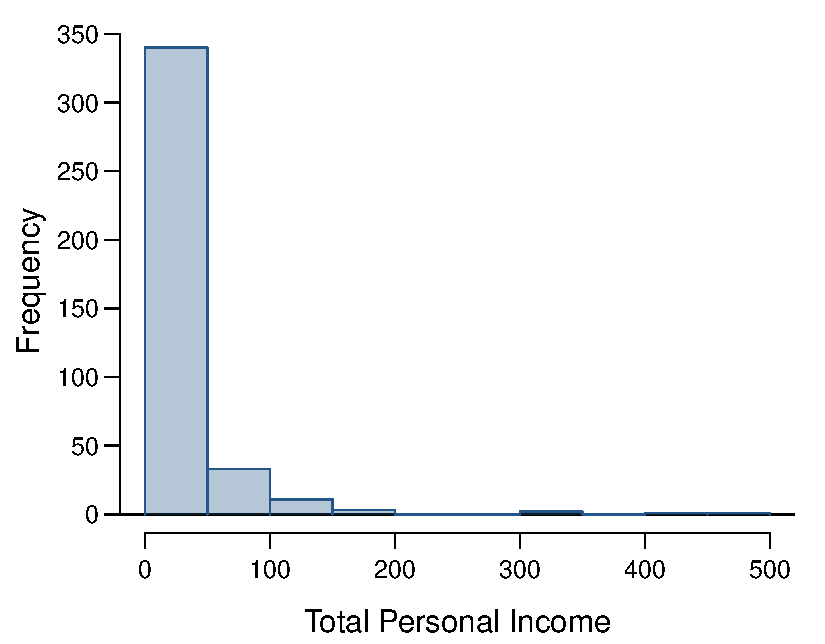
\includegraphics[width=\textwidth]{02/figures/eoce/TotalPersonalIncome.pdf}
\end{center}
\end{minipage}
\begin{minipage}[c]{0.38\textwidth}
{\small
\begin{center}
\begin{tabular}{cr}
  \hline
\textit{Income} & \textit{Frequency} \\ 
  \hline
0 - 50,000 & 340 \\ 
  50,001 - 100,000 & 33 \\ 
  100,001 - 150,000 & 11 \\ 
  150,001 - 200,000 & 3 \\ 
  200,001 - 250,000 & 0 \\ 
  250,001 - 300,000 & 0 \\ 
  300,001 - 350,000 & 2 \\ 
  350,001 - 400,000 & 0 \\ 
  400,001 - 450,000 & 1 \\ 
  450,001 - 500,000 & 1 \\ 
   \hline
\end{tabular}
\end{center}
}
\end{minipage} \\

\begin{minipage}[c]{0.6\textwidth}
\begin{center}
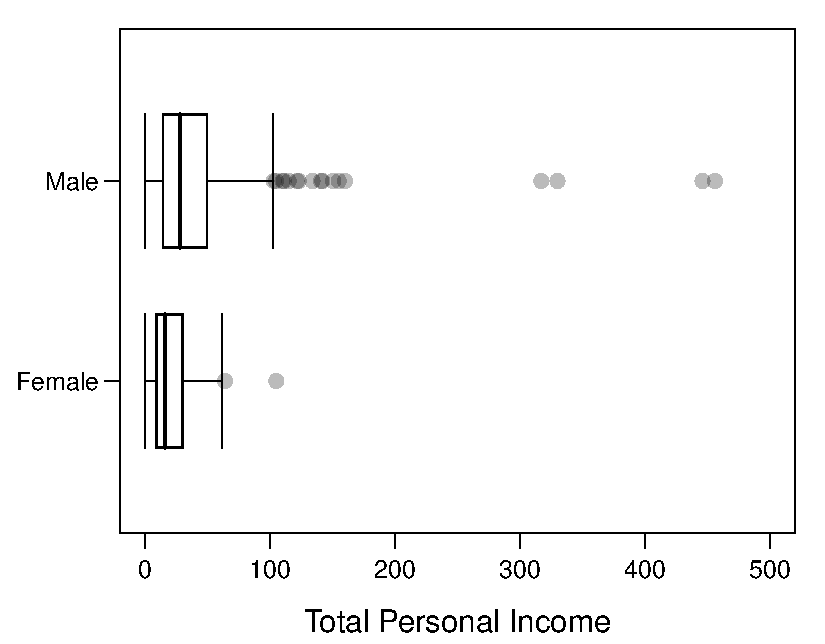
\includegraphics[width=\textwidth]{02/figures/eoce/TotalPersonalIncomeGender.pdf}
\end{center}
\end{minipage}
\begin{minipage}[c]{0.3\textwidth}
{\small
\begin{center}
\begin{tabular}{lr}
  \hline
Gender & Frequency \\ 
  \hline
Female & 188 \\ 
  Male & 203 \\ 
   \hline
\end{tabular}
\end{center}
}
\end{minipage}
}
{
\begin{enumerate}[(a)]
\item The distribution is right skewed, with a median between 0 and 50,000. Values range from 0 to 500,000 and there are potential outliers on the higher end. 
\item P(less than \$50,000) = 340 / 391 = 0.8696
\item P(female) = 188 / 391 = 0.4808
\item P(less than \$50,000 and female) = P(less than \$50,000) * P(female) = 0.4181
\item Probably not. It appears that females on average make less money than men. Also many men have a total personal income that may be considered an outlier, while only two women do.
\end{enumerate}
}

%%%%%%%%%%%%%%%%%%%%%%%%%%%%%%%%%%%%%

\subsection{Conditional probability}

%%%%%%%%%%%%%%%%%%%%%%%%%%%%%%%%%%%%%

% Independence, conditional

\eoce{P(A) = 0.3, P(B) = 0.7
\begin{enumerate}[(a)]
\setlength{\itemsep}{0mm}
\item Can you compute P(A and B) if you only know P(A) and P(B)?
\item Assuming that events A and B arise from independent random processes,
\begin{multicols}{3}
\begin{enumerate}[(i)]
\item what is P(A and B)?
\item what is P(A or B)?
\item what is P(A$|$B)?
\end{enumerate}
\end{multicols}
\item If we are given that P(A and B) = 0.1, are the random variables giving rise to events A and B independent?
\item If we are given that P(A and B) = 0.1, what is P(A$|$B)?
\end{enumerate}
}
{
\begin{enumerate}[(a)]
\item We cannot compute $P(A \cap B)$ since we do not know if A and B are independent.
\item
\begin{enumerate}[(i)]
\item If we know that A and B are independent, P(A and B) = P(A) * P(B) = 0.21.
\item P(A or B) = P(A) + P(B) - P(A and B) =  0.3 + 0.7 - 0.21 = 0.79.
\item If we know that A and B are independent, P(A$|$B) = P(A) = 0.3. 
\end{enumerate}
\item No because 0.1 $\ne$ 0.21.
\item P(A$|$B) = P(A and B) / P(B) = 0.1 / 0.7 = 0.143.
\end{enumerate}
}

% Cameras - indepedence

\eoce{Based on the probabilities provided in Exercise~\eoceref{cameras}, are the variables owning a DSLR and owning a point-and-shoot camera independent?}
{
If P(DSLR $|$ point-and-shoot) = P(DSLR), then the variables owning a DSLR and point-and-shoot are independent. So let's check if that's the case. \\
\begin{align*}
P(DSLR | point\&shoot) &= \frac{P(DSLR~and~point\&shoot)}{P(point\&shoot)} \\
&= \frac{0.20}{0.90} \\
&= 0.22
\end{align*}
Since 0.22 $\ne$ P(DSLR), the two variables are not independent.
}

% Languages - indepedence

\eoce{Based on the probabilities provided in Exercise~\eoceref{languages}, are the variables speaking French and speaking Spanish independent?}
{
If P(Spanish $|$ French) = P(Spanish), then the variables speaking French and speaking Spanish independent. So let's check if that's the case. \\
\begin{align*}
P(Spanish | French) &= \frac{P(Spanish~and~ French)}{P(French)} \\
&= \frac{0.20}{0.45} \\
&= 0.44
\end{align*}
Since 0.44 $\ne$ P(Spanish), the two variables are not independent.
}

% Contingency table (German men)

\eoce{Exercise~\ref{GermanMen} introduces a contingency table summarizing the relationship between hair color and eye color for a group of 1,770 German men. Answer the following questions based on this table.
\begin{enumerate}[(a)]
\setlength{\itemsep}{0mm}
\item What is the probability that a randomly chosen man has black hair?
\item What is the probability that a randomly chosen man has black hair given that he has blue eyes?
\item What is the probability that a randomly chosen man has black hair given that he has brown eyes?
\item Are hair color and eye color independent?
\end{enumerate}
}
{
\begin{enumerate}[(a)]
\item P(black hair) = 500 / 1770 = 0.2825
\item P(black hair $|$ brown eyes) = 300 / 720 = 0.4167
\item P(black hair $|$ blue eyes) = 200 / 1050 = 0.1905
\item No because P(black hair $|$ brown eyes) $ne$ P(black hair $|$ blue eyes), i.e. it is not equally likely for brown eyed and blue eyed men to have black hair.
\end{enumerate}
}

% Contingency table (cars)

\eoce{The below contingency table on the type and drive train of cars has been constructed based on the \texttt{cars} data set used introduced in Chapter 1. Answer the following questions based on this table.
\begin{center}
\begin{tabular}{lrrrr}
& & \multicolumn{3}{c}{\textit{Drive Train}} \\
\cline{3-5}
& & 4WD & front & rear \\ 
\cline{2-5}
& large &   0 &   7 &   4 \\ 
\textit{Type} &  midsize &   0 &  17 &   5 \\ 
& small &   2 &  19 &   0 \\ 
\cline{2-5}
\end{tabular}
\end{center}
\begin{enumerate}[(a)]
\setlength{\itemsep}{0mm}
\item What is the probability that a randomly chosen car is midsize?
\item What is the probability that a randomly chosen car has front wheel drive?
\item What is the probability that a randomly chosen car has front wheel drive and is midsize?
\item What is the probability that a randomly chosen car has front wheel drive given that it is midsize?
\item What is the marginal distribution of drive train?
\item What is the conditional distribution of drive train for midsize cars, i.e. what are the conditional probabilities is of 4WD, front wheel drive and rear wheel drive when given that the car is midsize?
\item Are type and drive train independent? Would you be comfortable generalizing your conclusion to all cars?
\end{enumerate}
}
{
\begin{enumerate}[(a)]
\item P(midsize) = (17 + 5) / 54 = 0.4074
\item P(front wheel drive) = (19 + 17 + 7) / 54 = 0.7963
\item P(front wheel drive and midsize) = 17 / 54 = 0.3148
\item P(front wheel drive $|$ midsize) = 17 / (17 + 5) = 0.7727
\item The marginal distribution of drive train is as follows: \\

\begin{tabular}{r | l}
Drive Train & Probability \\
\hline
4WD		& 2 / 54 = 0.0370 \\
front		& 43 / 54 = 0.7963 \\
rear		& 9 / 54 = 0.1667
\end{tabular}
\item[(f)] The conditional distribution of drive train is as follows: \\

\begin{tabular}{r | l}
\multicolumn{2}{c}{Type = midsize} \\
\hline
DT & Probability \\
\hline
4WD		& 0 \\
front		& 17 / 22 = 0.7727 \\
rear		& 5 / 22 = 0.2273
\end{tabular}

\item It appears that type and drive train are not independent since the conditional distribution of drive train is different for each type of car. For example, while only about 63\% of large cars have front wheel drive, a higher percentage of midsize cars (about 77\%) and an even higher percentage of small cars (about 90\%) have front wheel drive. However it should be noted that the sample size is quite small (only 54 cars) therefore we may not be comfortable generalizing our conclusions to all cars.
\end{enumerate}
}

% Probabilities (contingency table)

\eoce{A survey conducted in 2010 by Survey USA for KABC-TV Los Angeles asked 500 Los Angeles residents ``What is the best hamburger place in Southern California? Five Guys Burgers? In-N-Out Burger? Fat Burger? Tommy's Hamburgers? Umami Burger? Or somewhere else?" Consider the results of this survey, shown in the table below, in each of the following questions.
\begin{center}
\begin{tabular}{l p{4cm} r r r }
&						& \multicolumn{2}{c}{\textit{Gender}} \\
\cline{3-4}
&								& Male	& Female 	& Total\\
\cline{2-5}
& Five Guys Burgers					&5		&6	 	& 11	\\
& In-N-Out Burger					&162	&181	& 343 \\
\textit{Best} & Fat Burger				&10		&12	 	& 22 \\
\textit{hamburger} & Tommy's Hamburgers	&27		&27	 	& 54	\\ 
\textit{place} & Umami Burger			&5		&1	 	& 6 \\
& Other							&26		&20	 	& 46 \\
& Not Sure						&13		&5	 	& 18 \\
\cline{2-5}
&Total							&248	&252	& 500
\end{tabular}
\end{center}
\begin{enumerate}[(a)]
\setlength{\itemsep}{0mm}
\item What is the probability that a randomly chosen male likes In-N-Out the best?
\item What is the probability that a randomly chosen female likes In-N-Out the best?
\item What is the probability that a man and a woman who are dating both like In-N-Out the best?
\item What assumption did you make to calculate the probability in part (c)? Do you think this assumption is reasonable? 
\item What is the probability that a randomly chosen person likes Umami best or that person is female?
\end{enumerate}
}
{
\begin{enumerate}[(a)]
\item P(In-N-Out $|$ male) = 162 / 248 $\approx$ 0.65.
\item P(In-N-Out $|$ female) = 181 / 252 $\approx$ 0.72.
\item P(man and woman dating both like In-N-Out burgers the best) = 0.65 * 0.72 = 0.468.
\item We assumed that the burger preferences of the man and the woman are independent. This may not be a reasonable assumption since people tend to date people with similar likes/dislikes.
\item P(Umami or female) = P(Umami) + P(female) - P(Umami and female) = (6 / 500) + (252 / 500) - (1 / 500) = 0.514.
\end{enumerate}
}


% Probabilities (contingency table)

\eoce{A Pew Research poll conducted in October 2010 asked respondents ``From what you've read and heard, is there solid evidence that the average temperature on earth has been getting warmer over the past few decades, or not?". The contingency table below shows the distribution of responded with party and ideology \citep{globalWarming}.
\begin{center}
\begin{tabular}{ll  ccc c} 
							&						& \multicolumn{3}{c}{\textit{Response}} \\
\cline{3-5}
							&						& Earth is 		& Not 		& Don't Know	&	\\
							&						& warming	& warming 	& Refuse		& Total\\
\cline{2-6}
										& Conservative Republican	& 146	 	& 265		& 31 			& 442 	\\
\emph{Party and}							& Mod/Lib Republican		& 77	 		& 68 	 		& 16 			& 161 \\
\emph{Ideology}							& Mod/Cons Democrat		& 325	 	& 84 	 		& 31 			& 440 \\
							& Liberal Democrat			& 234	 	& 18 	 		& 11 			& 263 \\
\cline{2-6}
							&Total					& 782		& 435		& 89			& 1306
\end{tabular}
\end{center}
\begin{enumerate}[(a)]
\setlength{\itemsep}{0mm}
\item What is the probability that a randomly chosen respondent believes that the earth is warming?
\item What is the probability that a randomly chosen respondent is a liberal Democrat?
\item What is the probability that a randomly chosen respondent believes that the earth is warming and is a liberal Democrat?
\item What is the probability that a randomly chosen respondent believes the earth is warming or is a liberal Democrat?
\item What is the probability that a randomly chosen respondent believes the earth is warming given that s/he is a liberal Democrat?
\item What is the probability that a randomly chosen respondent believes that the earth is warming given that s/he is a conservative Republican?
\item Does it appear that whether or not a respondent believes that the earth is warming is independent of his/her party and ideology? Explain your reasoning.
\item What is the probability that a randomly chosen respondent is a moderate/liberal Republican given that s/he does not believe that the earth is warming? 
\end{enumerate}
}
{
\begin{enumerate}[(a)]
\item P(earth is warming) = $\frac{782}{1306} = 0.60$
\item P(liberal Democrat) = $\frac{263}{1306} = 0.20$
\item P(earth is warming and liberal Democrat) = $\frac{234}{1306} = 0.18$
\item P(earth is warming or liberal Democrat) = \\
= P(earth is warming) + P(liberal Democrat)  - P(earth is warming and liberal Democrat) \\
= 0.60 + 0.20 - 0.18 = 0.62
\item P(earth is warming $|$ liberal Democrat) = $\frac{234}{263} = 0.89$
\item P(earth is warming $|$ conservative Republican) = $\frac{146}{442} = 0.33$
\item No, the two appear to be dependent. The percentages of conservative Republicans and liberal Democrats who believe that there is solid evidence that the average temperature on earth has been getting warmer over the past few decades are very different.
\item P(moderate/liberal Republican $|$ not warming) = $\frac{68}{161} = 0.42$
\end{enumerate}
}


% Cats Body Weights Gender

\eoce{Exercise~\eoceref{catsBodyWeights} introduces a data set of of 144 cats' body weights and Exercise~\eoceref{catsBodyWeightsGender} shows the distribution of gender in this sample of 144 cats. If a randomly chosen cat weighs less than 2.5 \textit{kg}, is it more likely to be male or female?
}
{
In order to answer this question we need to compare P(female $|$ $<$ 2.5\textit{kg}) and P(male $|$ $<$ 2.5\textit{kg}).
\begin{align*}
P(female\text{ }| < 2.5 kg) &= P(female\text{ }and\text{ }< 2.5 kg)  / P(< 2.5 kg)  = 36 / (36 + 25) = 0.5902 \\
P(male\text{ }| < 2.5 kg) &= P(male\text{ }and\text{ }< 2.5 kg)  / P(< 2.5 kg)  = 25 / (36 + 25) = 0.4098
\end{align*}
Since P(female $|$ $<$ 2.5 kg) is greater than P(male $|$ $<$ 2.5 kg), the cat is more likely to be female.
}

% Probability tree (test)

\eoce{Suppose that a student is about to take a multiple choice test that covers algebra and trigonometry. 40\% of the questions are algebra and 60\% are trigonometry. There is a 90\% chance that she will get an algebra question right, and a 35\% chance that she will get a trigonometry question wrong.
\begin{enumerate}[(a)]
\setlength{\itemsep}{0mm}
\item If we choose a question at random from the exam, what is the probability that she will get it right?
\item If we choose a question at random from the exam, what is the probability that she will get it wrong?
\item If we choose a question at random from the exam, what is the probability that it will be an algebra question given that she got it wrong?
\end{enumerate}
}
{
\begin{multicols}{2}
\begin{center}
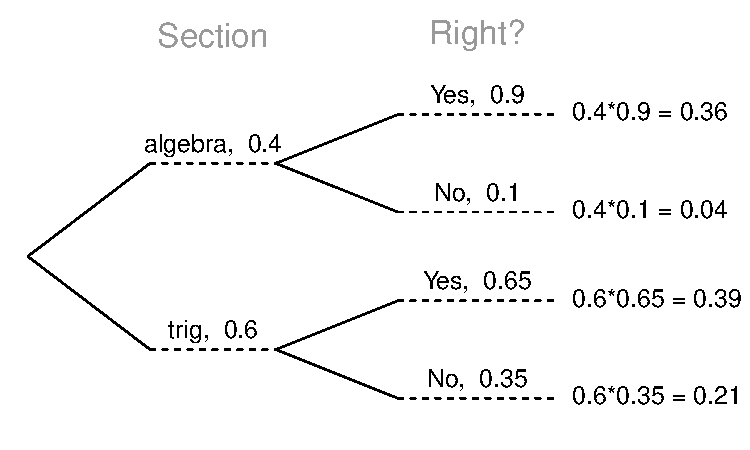
\includegraphics[width=70mm]{02/figures/eoce/algebraTrigTree.pdf}
\end{center}
\begin{enumerate}[(a)]
\item P(right) \\
 = P(right and algebra) + P(right and trig) \\
 = 0.36 + 0.39 = 0.75
\item P(wrong) = 1 - P(right) = 1 - 0.75 = 0.25
\item P(algebra $|$ wrong) \\
= $\frac{\text{P(algebra and wrong)}}{\text{P(wrong)}} = \frac{0.04}{0.25} = 0.16$
\end{enumerate}
\end{multicols}
}

% Probability tree (thrombosis)

\eoce{A genetic test is used to determine if people have a genetic predisposition for \textit{thrombosis}, formation of a blood clot inside a blood vessel that obstructs the flow of blood through the circulatory system. It is believed that 3\% of the people actually have this predisposition. This test is 99\% accurate if a person actually has the predisposition, meaning that the probability of a positive test result when a person actually has the predisposition is 0.99. The test is 98\% accurate if a person does not have the predisposition, meaning that the probability of a negative test result when a person does not actually have the predisposition is 0.98. What is the probability that a randomly selected person who is identified as having the predisposition by the test actually has the predisposition?}
{
\begin{multicols}{2}
\begin{center}
\includegraphics[width=70mm]{02/figures/eoce/thrombosisTree.pdf}
\end{center}
\begin{align*}
P(pre | positive) &= \frac{P(\text{pre and positive})}{P(positive)} \\
&= \frac{0.0297}{0.0297 + 0.0194} \\
&= 0.6049
\end{align*}
\end{multicols}
}

% Probability tree (lupus)

\eoce{Lupus is a medical phenomenon where antibodies that are supposed to attack foreign cells to prevent infections instead see plasma proteins as foreign bodies, leading to a high risk of clotting. It is believed that 2\% of the population suffer from this disease. 

The test for lupus is very accurate if the person actually has lupus, however is very inaccurate if the person does not. More specifically, the test is 98\% accurate if a person actually has the disease, meaning that the probability of a positive test result when a person actually has lupus is 0.98. The test is 74\% accurate if a person does not have the disease, meaning that the probability of a negative test result when a person does not actually have lupus is 0.74. 

Dr. Gregory House's team presents him a case where the patient tested positive for lupus. However Dr. House claims that ``It's never lupus", even though the test result is positive. What do you think? (\textit{Hint: What is the probability that a person who tested positive actually has lupus?})
}
{
\begin{multicols}{2}
\begin{center}
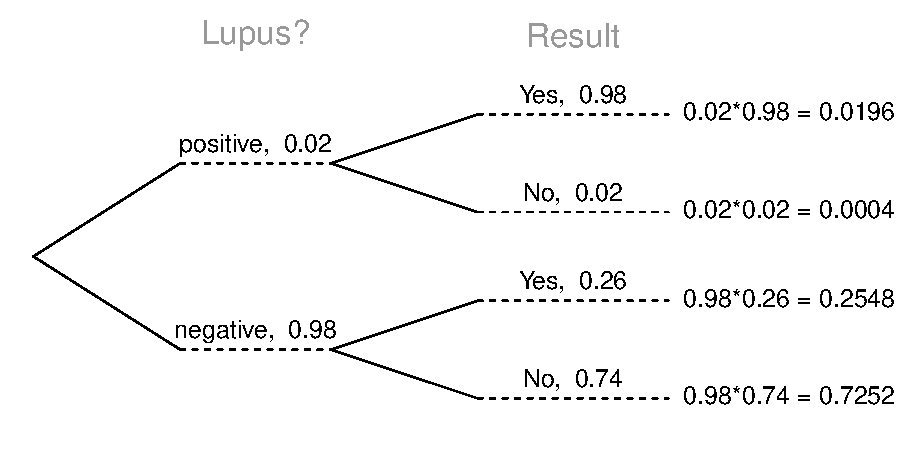
\includegraphics[width=70mm]{02/figures/eoce/lupusTree.pdf}
\end{center}
\begin{align*}
P(lupus | positive) &= \frac{P(lupus \cap positive)}{P(positive)} \\
&= \frac{0.0196}{0.0196 + 0.2548} \\
&= 0.0714
\end{align*}
Even when a patient tests positive for lupus, there is only a 7.14\% chance that he/she actually has lupus. House may be right.
\end{multicols}
}

% Probability tree (mammograms)

\eoce{In November 2009, the US Preventive Services Task Force changed its recommendations for breast cancer screening \citep{USPSTF:2009}. One of the reasons for this change was the high rate of false positives. Among many on this issue, an opinion piece which attempted to describe to the public how to calculate false positive rates was published in the New York Times \citep{Paulos:13Dec2009}. Below is an excerpt from the article:
\begin{adjustwidth}{2em}{2em}
``Assume there is a screening test for a certain cancer that is 95 percent accurate; that is, if someone has the cancer, the test will be positive 95 percent of the time. Let's also assume that if someone doesn't have the cancer, the test will be positive just 1 percent of the time. Assume further that 0.5 percent - one out of 200 people - actually have this type of cancer. Now imagine that you've taken the test and that your doctor somberly intones that you�ve tested positive. Does this mean you're likely to have the cancer? Surprisingly, the answer is no."
\end{adjustwidth}
\begin{enumerate}[(a)]
\setlength{\itemsep}{0mm}
\item Construct a tree diagram of this scenario.
\item Calculate the false positive rate for such a test, i.e. the probability that a person who tests positive does not actually have cancer.
\item Calculate the probability that a person who tests positive actually has cancer.
\end{enumerate}
}
{
\begin{multicols}{2}
\begin{enumerate}[(a)]
\item A tree diagram of this scenario is below:
\begin{center}
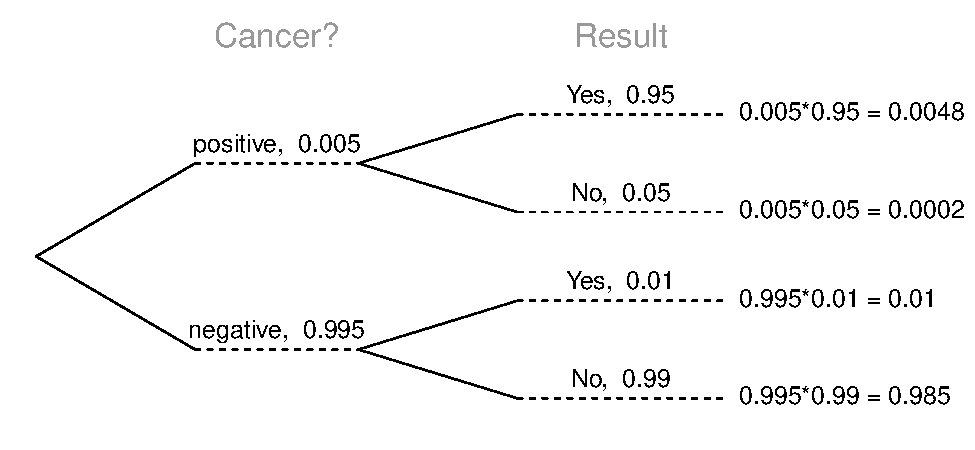
\includegraphics[width=60mm]{02/figures/eoce/cancerTree.pdf}
\end{center}
\item The calculation of the false positive rate is shown below:
\begin{align*}
P(no~cancer | positive) &= \frac{P(no~cancer~and~positive)}{P(positive)} \\
&= \frac{0.995 * 0.01}{0.005 * 0.95 + 0.995 * 0.01} \\
&= \frac{0.00995}{0.00475 + 0.00995} \approx 0.68
\end{align*}
\item P(cancer $|$ positive) \\
= 1 - P(no~cancer $|$ positive) \\
= 1 - 0.68 = 0.32.
\end{enumerate}
\end{multicols}
}\label{mammograms}


% Bayesian reasoning - mammograms

\eoce{Exercise~\eoceref{mammograms} gives the distribution of positive mammograms based on whether or not the patient actually has breast cancer. If a patient has a positive mammogram result would you guess she has cancer? What if she has a negative mammogram result? Explain your reasoning using the appropriate probabilities.}
{Since P(cancer $|$ positive) = 0.32 is a low probability, even if a woman has a positive mammogram result, it is unlikely that she actually has cancer. We also need to find P(cancer $|$ negative) in order to answer the rest of the question. 
\begin{align*}
P(cancer | negative) &= \frac{P(cancer~and~negative)}{P(negative)} \\
&= \frac{0.005 * 0.05}{0.005 * 0.05 + 0.995 * 0.99} \\
&= \frac{0.00025}{0.9853} \approx 0.0002537
\end{align*}
If a woman has a negative mammogram result, there is only a 0.03\% chance that she has cancer. That is a much lower probability, so we would guess she doesn't have cancer.}


% Probability tree (constructing box plots)

\eoce{After an introductory statistics course, 80\% of students can successfully construct box plots. Of those who can construct box plots, 86\% passed, while only 65\% of those students who could not construct box plots passed.
\begin{enumerate}[(a)]
\setlength{\itemsep}{0mm}
\item Construct a tree diagram of this scenario.
\item Calculate the probability that a student is able to construct a box plot if it is known that she passed.
\end{enumerate}
}
{
\begin{multicols}{2}
\begin{enumerate}[(a)]
\item A tree diagram of this scenario is below:
\begin{center}
\includegraphics[width=60mm]{02/figures/eoce/constructBoxPlot.pdf}
\end{center}
\item The calculation of the probability is shown below:
\begin{align*}
P(can~construct | pass) &= \frac{P(pass~and~can~construct)}{P(pass)} \\
&= \frac{0.80 * 0.86}{0.80 * 0.86 + 0.20 * 0.65} \\
&= \frac{0.688}{0.818} \approx 0.84
\end{align*}
\end{enumerate}
\end{multicols}
}\label{constructingBoxPlots}

% Bayesian reasoning - box plots

\eoce{Exercise~\eoceref{constructingBoxPlots} gives the distribution of statistics students who did and did not pass the course depending on whether or not they can successfully construct box plots. If a student can successfully construct box plots would you guess they did or did not pass the course? What if they can't successfully construct box plots? Explain your reasoning using the appropriate probabilities.}
{
Since P(can construct $|$ pass) = 0.84 is a high probability, if a student can successfully construct probability trees we would expect him/her to have passed the course. We also need to find P(can construct $|$ fail) in order to answer the rest of the question.
\begin{align*}
P(can~construct | pass) &= \frac{P(fail~and~can~construct)}{P(fail)} \\
&= \frac{0.80 * 0.14}{0.80 * 0.14 + 0.20 * 0.45} \\
&= \frac{0.112}{0.202} \approx 0.55
\end{align*}
If a student cannot successfully construct probability trees, there is only a 55\% chance that s/he would have passed. That is a lower probability, but it is not so low, so it would be difficult to guess if s/he passed or did not pass the course.}

%%%%%%%%%%%%%%%%%%%%%%%%%%%%%%%%%%%%%

\subsection{Sampling from a small population}

%%%%%%%%%%%%%%%%%%%%%%%%%%%%%%%%%%%%%

\eoce{Imagine you have an urn with 5 red, 3 blue and 2 orange marbles in it. 
\begin{enumerate}[(a)]
\setlength{\itemsep}{0mm}
\item What is the probability that the first marble you draw is blue?
\item Imagine you in fact drew a blue marble in the first draw. If drawing with replacement, what is the probability of drawing a blue marble in the second draw?
\item Imagine you instead drew an orange marble in the first draw. If drawing with replacement, what is the probability of drawing a blue marble in the second draw?
\item If drawing with replacement, what is the probability of drawing two blue marbles in a row?
\item When drawing with replacement does the color of the first marble you draw affect the probability of that the second marble you draw is blue? What does this say about whether or not the draws are independent?
\end{enumerate}
}
{
\begin{enumerate}[(a)]
\item $P(1^{st} \text{ marble } B) = \frac{3}{5 + 3 + 2} = \frac{3}{10} = 0.3$
\item $P(2^{nd} \text{ marble } B | 1^{st} \text{ marble } B) = \frac{3}{10} = 0.3$
\item $P(2^{nd} \text{ marble } B | 1^{st} \text{ marble } O) = \frac{3}{10} = 0.3$
\item $P(1^{st} \text{ marble } B) \cdot P(2^{nd} \text{ marble } B | 1^{st} \text{ marble } B) = 0.3 * 0.3 = 0.09$
\item When drawing with replacement, probability of the second marble being blue does not depend on the color of the first marble since whatever we draw in the first draw gets put back in the urn. For example $P(B | B) = P(B | O)$. Therefore, when drawing with replacement, draws are independent.
\end{enumerate}
}\label{urnWithMarbles}

%

\eoce{Imagine the same urn from Exercise~\eoceref{urnWithMarbles} with 5 red, 3 blue and 2 orange marbles in it. You just drew one marble from the urn and you are about to find out what color it is.
\begin{enumerate}[(a)]
\setlength{\itemsep}{0mm}
\item Imagine you drew a blue marble in the first draw. If drawing without replacement, what is the probability of drawing a blue marble in the second draw?
\item Imagine you instead drew an orange marble in the first draw. If drawing without replacement, what is the probability of drawing a blue marble in the second draw?
\item If drawing without replacement, what is the probability of drawing two blue marbles in a row?
\item When drawing without replacement does the color of the first marble you draw affect the probability of that the second marble you draw is blue? What does this say about whether or not the draws are independent?
\end{enumerate}
}
{
\begin{enumerate}[(a)]
\item $P(2^{nd} \text{ marble } B | 1^{st} \text{ marble } B) = \frac{2}{9} = 0.22$
\item $P(2^{nd} \text{ marble } B | 1^{st} \text{ marble } O) = \frac{3}{9} = 0.33$
\item $P(1^{st} \text{ marble } B) \cdot P(2^{nd} \text{ marble } B | 1^{st} \text{ marble } B)  = 0.3 * 0.22 = 0.066 $
\item When drawing with replacement, probability of the second marble being blue does depend on the color of the first marble since whatever we draw in the first draw gets put back in the urn. For example $P(B | B) \ne P(B | O)$. Therefore, when drawing with replacement, draws are dependent.
\end{enumerate}
}

%

\eoce{In your sock drawer you have 4 blue socks, 5 grey socks, and 3 black ones. Half asleep one morning you grab 2 socks at random and put them on. Find the probability you end up wearing
\begin{multicols}{3}
\begin{enumerate}[(a)]
\setlength{\itemsep}{0mm}
\item 2 blue socks
\item no grey socks
\item at least 1 black sock
\item a green sock
\item matching socks
\end{enumerate}
\end{multicols}
}
{
\begin{enumerate}[(a)]
\item \underline{Blue} \underline{Blue} $\rightarrow \frac{4}{12} * \frac{3}{11} = 0.0909$
\item \underline{Not Gray} \underline{Not Gray} $\rightarrow \frac{7}{12} * \frac{6}{11} = 0.3182$
\item P(at least 1 black) = 1 - P(no black) \\
P(no black) $\rightarrow$  \underline{Not Black} \underline{Not Black} $\rightarrow \frac{9}{12} * \frac{8}{11} = 0.5455$ \\
P(at least 1 black) = 1 - 0.5455 = 0.4545
\item 0, there are no green socks in the drawer.
\item \underline{Blue} \underline{Blue} $\rightarrow 0.0909$ \\
\underline{Black} \underline{Black} $\rightarrow \frac{3}{12} * \frac{2}{11} = 0.0455$ \\
\underline{Gray} \underline{Gray} $\rightarrow \frac{5}{12} * \frac{4}{11} = 0.1515$ \\
P(matching socks) = 0.0909 + 0.0455 + 0.1515 = 0.2879
\end{enumerate}
}

%

\eoce{The table below shows the distribution of books in your bookcase based on whether they are non-fiction or fiction and hardcover or paperback. Suppose you randomly draw two books from your shelf, without replacement. For simplicity, suppose you draw them one-at-a-time. Calculate the probability that the books are as follows.
\begin{center}
\begin{tabular}{ll  cc c} 
							&			& \multicolumn{2}{c}{\textit{Format}} \\
\cline{3-4}
							&			& Hardcover 	& Paperback 	& Total	\\
\cline{2-5}
\multirow{2}{*}{\textit{Type}}		&Fiction 		& 13	 		& 59			& 72 	\\
							&Non-fiction	& 15	 		& 8 	 		& 23 \\
\cline{2-5}	
							&Total		& 28			& 67			& 95
\end{tabular}
\end{center}
\begin{enumerate}[(a)]
\setlength{\itemsep}{0mm}
\item Both books are fiction.
\item The first book you draw is a hardcover fiction and the second is a paperback fiction.
\item The first book you draw is a hardcover and the second is a paperback.
\item The first book is a hardcover or a fiction book. The second book can be anything.
\item At least one of the books is a paperback.
\end{enumerate}
}
{
\begin{enumerate}[(a)]
\item P(both fiction) = $\frac{72}{95} * \frac{71}{94} = 0.5724$
\item P(first hardcover fiction, second paperback fiction) = $\frac{13}{95} * \frac{59}{94} = 0.0859$
\item P(first hardcover, second paperback) = $\frac{28}{95} * \frac{67}{94} =  0.2101$
\item P(first book is a hardcover or a fiction, second anything) \\
= [P(hardcover) + P(fiction) - P(hardcover and fiction)] * P(any) \\
= $\left( \frac{28}{95} + \frac{72}{95} - \frac{13}{95} \right) * 1 = 0.9158$
\item P(two books at least one of which is paperback) = 1 - P(no paperbacks in two books) = $1 - \left(\frac{28}{95} * \frac{27}{94} \right) = 1 - 0.0847 = 0.9153$
\end{enumerate}
}

%

\eoce{In a classroom with 24 students, 7 students are wearing jeans, 4 students are wearing shorts, 8 students are wearing skirts, and the rest are wearing leggings. If we randomly select 3 students without replacement, what is the probability that one of the selected students is wearing leggings and the other two are wearing jeans?}
{
The number of students wearing leggings is $24 - (7+4+8) = 5$. When selecting 3 students, there are three scenarios under which we would get one student with leggings and two with jeans: \\
\begin{center}
Scenario 1 = P(L,J,J) = $\frac{5}{24} * \frac{7}{23} * \frac{6}{22} = 0.0173$ \\
Scenario 2 = P(J,L,J) = $\frac{7}{24} * \frac{5}{23} * \frac{6}{22} = 0.0173$ \\
Scenario 3 = P(J,J,L) = $\frac{7}{24} * \frac{6}{23} * \frac{5}{22} = 0.0173$ \\
\end{center}
These scenarios exhaust the ways where we can get one student with leggings and two students with jeans, and these scenarios are also disjoint. Therefore, to determine the probability that one of the selected students is wearing leggings and the other two are wearing jeans we simply add up the calculated probabilities:
\[ 0.0173 + 0.0173 + 0.0173 = 0.0519 \]
Note that each scenario has the same probability.
}

%

\eoce{Suppose we pick three people at random. For each of the following questions, ignore the special case where someone might be born on February 29th.
\begin{enumerate}[(a)]
\setlength{\itemsep}{0mm}
\item What is the probability that the first two people share a birthday? 
\item What is the probability that at least one pair of people share a birthday?
\end{enumerate}
}
{
\begin{enumerate}[(a)]
\item P(first two people share a birthday) = 1/365 = 0.0027.
\item P(at least one pair of people share a birthday) \\
= 1- P(none of the three people share a birthday) = 1 - (365/365)(364/365)(363/365) = 0.0082.
\end{enumerate}
}


%%%%%%%%%%%%%%%%%%%%%%%%%%%%%%%%%%%%%

\subsection{Expected value and uncertainty}

%%%%%%%%%%%%%%%%%%%%%%%%%%%%%%%%%%%%%

\eoce{At a university 13\% of students smoke.
\begin{enumerate}[(a)]
\setlength{\itemsep}{0mm}
\item Calculate the expected number of smokers in a random sample of 100 students from this university.
\item The university gym opens at 9am on Saturday mornings. On a Saturday morning at 8:55am there are 27 students waiting outside the gym for it to open. Should you use the same approach from part (a) to calculate the expected number of smokers among these 27 students?
\end{enumerate}
}
{
\begin{enumerate}[(a)]
\item E(X) = 100 * 0.13 = 13
\item No, these 27 students are not a random sample from the university's student population. Chances are the proportion of smokers among students who go to the gym, let alone those who go at 9am on a Saturday morning, is much lower than the proportion of smokers in the university as a whole.
\end{enumerate}
}

%

\eoce{You draw a card from a deck. If you get a red card, you win nothing. If you get a spade, you win \$5. For any club, you win \$10 plus an extra \$20 for the ace of clubs.
\begin{enumerate}[(a)]
\setlength{\itemsep}{0mm}
\item Create a probability model for the amount you win at this game and find the expected winnings and the standard deviation of the expected winnings.
\item What is the maximum amount you would be willing to pay to play this game? In other words, what would be the cost of this game to make it fair?
\end{enumerate}
}
{
\begin{enumerate}[(a)]
\item The probability model and the calculation of the expected value and standard deviation are shown below:
\begin{center}
\renewcommand{\arraystretch}{1.5}
\begin{tabular} { l | l | l | l | l | l}
Event 	& $X$ & $P(X)$ 	& $X \cdot P(X)$ 	& $(X - E(X))^2$	& $(X - E(X))^2 \cdot P(X)$ \\
\hline
Red		&0 & $\frac{26}{52}$ 		& $0 * \frac{26}{52} = 0$		& $(0 - 4.14)^2 = 17.1396$	
	& $17.1396 * \frac{26}{52} =  8.5698$ \\
Spade	&5 & $\frac{13}{52}$ 		& $5 * \frac{13}{52} = 1.25$ 	& $(5 - 4.14)^2 = 0.7396$
	& $0.7396 * \frac{13}{52} = 0.1849$ \\
Club		&10 & $\frac{12}{52}$ 		& $10 * \frac{12}{52} = 2.31$	& $(10 - 4.14)^2 = 34.3396$
	& $34.3396 * \frac{12}{52} = 7.9245$ \\
Ace of clubs	&30 & $\frac{1}{52}$ 	& $30 * \frac{1}{52} = 0.58$	& $(30 - 4.14)^2 = 668.7396$
	& $668.7396 * \frac{1}{52} = 12.8604$ \\
\hline
&&& $E(X) = 4.14$	& 	& $V(X) = 29.5396$ \\
\multicolumn{5}{l |}{}  		& $SD(X) = \sqrt{V(X)} = 5.4350$
\end{tabular}
\end{center}
\item You should not be paying more than the expected value of the game, therefore you should be willing to pay up to \$4.14.
\end{enumerate}
}

%

\eoce{In a card game you start with a well shuffled full deck and draw 3 cards without replacement. If you draw 3 hearts in a row, you win \$50. If you draw 3 black cards, you win \$25. For any other draws you win nothing.
\begin{enumerate}[(a)]
\setlength{\itemsep}{0mm}
\item Create a probability model for the amount you win at this game and find the expected winnings. Also verify the standard deviation of this distribution is \$3.37.
\item If the game costs \$5 to play, what would be the expected value and standard deviation of net profit (or loss)? \textit{(Hint: profit = winnings $-$ cost; $X-5$)}
\item If the game costs \$5 to play, should you play this game? Why or why not? Explain.
\end{enumerate}
}
{
\begin{enumerate}[(a)]
\item The probability model and the calculation of the expected value are shown below:
\begin{adjustwidth}{-5em}{-5em}
\begin{center}
\renewcommand{\arraystretch}{1.5}
\begin{tabular} { l | l | l | l | l | l}
Event 	& X		& P(X)										& X * P(X) 	& $(X - E(X))^2$	& $(X - E(X))^2 \cdot P(X)$ \\
\hline
3 hearts	& 50		& $\frac{13}{52} * \frac{12}{51} * \frac{11}{50} = 0.0129$	& 0.65		& $(0.65 - 3.59)^2 = 8.6436 $	& $8.6436 * 0.0129 = 0.1115$ 	 \\
3 blacks	& 25		& $\frac{26}{52} * \frac{25}{51} * \frac{24}{50} = 0.1176$	& 2.94		& $(2.94 - 3.59)^2 = 0.4225 $	& $0.4225 * 0.1176 = 0.0497$  \\
Else		& 0		& $1 - (0.0129 + 0.1176) = 0.8695$					& 0 			& $(0 - 3.59)^2 = 12.8881 $	& $12.8881 * 0.8695 = 11.2062$ \\
\hline
		&		&											& E(X) = \$3.59 & 						& $V(X) = 11.3674 $ \\
\multicolumn{5}{l |}{}  																				& $SD(X) = \sqrt{V(X)} = 3.37$
\end{tabular}
\end{center}
\end{adjustwidth}
\item Let $X$ denote winnings, then net profit can be denoted as $X - 5$.
\begin{align*}
E(X - 5) &= E(X) - 5 = 3.59 - 5 = \$-1.41 \\
SD(X - 5) &= SD(X) = 3.37
\end{align*}
\item No, the expected net profit is negative so on average you expect to lose money.
\end{enumerate}
}

%

\eoce{In the game of roulette, a wheel is spun and you place bets on where the marble will stop. One popular bet is that it will stop on a red slot. Each slot is equally likely. There are 38 slots, and 18 of them are red. If it does stop on red, you win \$1. If not, you lose \$1.
\begin{enumerate}[(a)]
\setlength{\itemsep}{0mm}
\item Let X represent the amount you win/lose on a single spin. Write a probability model for X.
\item What's the expected value and standard deviation of your winnings?
\end{enumerate}
}
{
\begin{enumerate}
\item The probability model for X is as follows: \\
\renewcommand{\arraystretch}{1.5}
\begin{tabular} {c|c}
X & P(X) \\
\hline
1 & $\frac{18}{38}$ \\
-1 & $\frac{20}{38}$ \\
\end{tabular}

\item The expected value and the standard deviation of X can be calculated as follows:
\begin{center}
\renewcommand{\arraystretch}{1.5}
\begin{tabular} {l | l | l | l | l}
$X$ 	& $P(X)$ 			& $X \cdot P(X)$	& $(X - E(X))^2$	& $(X - E(X))^2 \cdot P(X)$ \\
\hline
1 	& $\frac{18}{38}$	& $1 * \frac{18}{38}  = \frac{18}{38}$	& $(1 + 0.0526)^2 = 1.1080$	& 
$1.1080 * \frac{18}{38} =  0.5248$\\
-1 	& $\frac{20}{38}$	& $-1 * \frac{20}{38}  = -\frac{20}{38} $ & $(-1 + 0.0526)^2 = 0.8976$ & $0.8976 * \frac{20}{38} =  0.4724$\\
\hline
	&				& $E(X) = - \frac{2}{38} = -0.0526$ & & $V(X) = 0.9972 $ \\
\multicolumn{4}{l |}{}  		& $SD(X) = \sqrt{V(X)} = 0.9986$
\end{tabular}
\end{center}
\end{enumerate}
}\label{roulette}

%

\eoce{Exercise~\eoceref{roulette} describes winnings on a game of roulette.
\begin{enumerate}[(a)]
\setlength{\itemsep}{0mm}
\item Suppose you play \$3 on roulette so winnings and losses are tripled. Let Y represent the total amount won or lost in this game. What is the expected value and standard deviation of your total winnings?
\item Suppose you play roulette 3 times, each time with \$1. Let W represent the total amount won or lost. What is the expected value and standard deviation of your total winnings?
\item How to your answers to parts (a) and (b) compare? What does this say about the riskiness of the two games?
\end{enumerate}
}
{
\begin{enumerate}[(a)]
\item Let $Y$ represent the winnings from a game where winnings and losses are tripled. Then, $Y = 3X$.
\begin{align*}
E(Y) &= E(3X) = 3 E(X) = 3 * -0.0526 = \$-0.16 \\
V(Y) &= V(3X) = 3^2 V(X) = 3^2 * 0.9986^2 = 8.9748 \\
SD(Y) &= \sqrt{V(Y)} = \sqrt{8.9748} = \$3.00
\end{align*}
\item Let $W$ represent the winnings from a three games. Then, $W = X + X + X$.
\begin{align*}
E(W) &= E(X + X + X) = E(X) +E(X) + E(X) = 3 E(X) = 3 * -0.0526 = \$-0.16 \\
SD(W) &= SD(X + X + X) = \sqrt{V(X) + V(X) + V(X)} = \sqrt{3 V(X)} = \sqrt{3 * 0.9972} = \$1.73
\end{align*}
\item Expected values are the same but the standard deviations are different. The standard deviation from the game where winnings and losses are tripled is higher, making this game riskier.
\end{enumerate}
}

%

\eoce{American Airlines charges the following baggage fees: \$20 for the first bag and \$30 for the second. Suppose 54\% of passengers have no checked luggage, 34\% have one piece of checked luggage and 12\% have two pieces. We suppose a negligible portion of people check more than two bags.
\begin{enumerate}[(a)]
\setlength{\itemsep}{0mm}
\item Build a probability model and compute the average revenue per passenger as well as the standard deviation.
\item About how much revenue should they expect for a flight of 120 passengers? With what standard deviation?
\end{enumerate}
}
{
\begin{enumerate}[(a)]
\item The probability model and the calculation of average revenue per passenger (expected value) are as follows:
\begin{center}
\renewcommand{\arraystretch}{1.5}
\begin{tabular} {l | l | l | l | l | l}
Event 					& X	& P(X)	& X * P(X) 	& $(X - E(X))^2$			& $(X - E(X))^2 * P(X)$ \\
\hline
No baggage 				& 0	& 0.54	& 0			& $(0 - 12.80)^2 = 163.84$	& 163.84 * 0.54 = 88.47  \\
1 checked bag				& 20	& 0.34	& 6.8 		& $(20 - 12.80)^2 = 51.84$	& 51.84 * 0.34 = 17.63 \\
2 checked bags			& 50	& 0.12	& 6 			& $(50 - 12.80)^2 = 1383.84$	& 1383.84 * 0.12 = 166.06 \\
\hline
						&	&		& E(X) = \$12.80	&	& V(X) = \$272.16 \\
\multicolumn{5}{l |}{}  										& $SD(X) = \sqrt{V(X)} = \$16.50$
\end{tabular}
\end{center}
\item $E(\underbrace{X + \cdots + X}_{120}) =  \underbrace{E(X) + \cdots + E(X)}_{120} = 120 * E(X) = 120 * 12.80 = \$1536$ \\
$V(\underbrace{X + \cdots + X}_{120}) =  \underbrace{V(X) + \cdots + V(X)}_{120} = 120 * V(X) = 120 * 272.16 = \$32659.20$ \\
$SD(\underbrace{X + \cdots + X}_{120}) = \sqrt{32659.20} = \$180.71$
\end{enumerate}
}\label{americanAir}


%

\eoce{Andy is always looking for ways to make money fast. Lately he has been trying to make money by gambling. Here is the game he is considering playing:

The game costs \$2 to play. He draws a card from a deck. If he gets a number card (2-10) he wins nothing. For any face card (jack, queen or king) he wins \$3, for any ace he wins \$5 and he wins an extra \$20 if he draws the ace of clubs.
\begin{enumerate}[(a)]
\setlength{\itemsep}{0mm}
\item Create a probability model for the amount he wins at this game and find his expected winnings.
\item Would you recommend this game to Andy as a good way to make money? Explain.
\end{enumerate}
}
{
\begin{enumerate}[(a)]
\item The probability model for the amount Andy can win at this game and the calculation of the expected winnings is as follows:
\begin{center}
\renewcommand{\arraystretch}{1.5}
\begin{tabular} {l | l | l | l}
Event 	& $X$ & $P(X)$ 	& $X \cdot P(X)$	  \\
\hline
Number	&-2 & $\frac{36}{52} = 0.6923$ 		& $-2 * \frac{36}{52} = -1.38$ 	  \\
J, Q, K	&1 & $\frac{12}{52} = 0.2308$ 		& $1 * \frac{12}{52} = 0.23$  \\
Ace		&3 & $\frac{3}{52} = 0.0577$		& $3 * \frac{3}{52} = 0.17$  \\
Ace of clubs	&23 & $\frac{1}{52} = 0.0192$ 	& $23 * \frac{1}{52} = 0.44$  \\
\hline
&&& $E(X) = -0.54$ 
\end{tabular}
\end{center}

\item No, he is expected to lose money on average.

\end{enumerate}
}

%

\eoce{A portfolio's value increases by 18\% during a financial boom and by 9\% during normal times while it decreases by 12\% during a recession. What is the expected return on this portfolio if each scenario is equally likely?}
{
\begin{center}
\renewcommand{\arraystretch}{1.5}
\begin{tabular} {l | l | l | l}
Event 		& $X$ 	& $P(X)$ 			& $X \cdot P(X)$	  \\
\hline
Boom		& 0.18	& $\frac{1}{3}$ 		& $0.18 * \frac{1}{3} = 0.06$ 	  \\
Normal		& 0.09	& $\frac{1}{3}$ 		& $0.09 * \frac{1}{3} = 0.03$  \\
Recession	& -0.12	& $\frac{1}{3}$		& $-0.12 * \frac{1}{3} = -0.04$  \\
\hline
&&& $E(X) = 0.05$ 
\end{tabular}
\end{center}
The expected return is a 5\% increase in value.
}


%

\eoce{You and your friend decide to bet on the Major League Baseball game happening one evening between the Los Angeles Dodgers and the San Diego Padres. Current standing statistics indicate that the Dodgers have 0.46 probability of winning this game against the Padres. If your friend bets you \$5 that the Dodgers will win, how much would you need to bet on the Padres to make this a fair game.}
{A fair game means an expected value of 0.
\begin{align*}
0 &= 5 * 0.46 + x * 0.54 \\
x &= -2.3 / 0.54 \\
x &\approx -4.26
\end{align*}
You would bet \$4.26 for the Padres to make the game fair.
}

%

\eoce{Marcie has been tracking the following two items on Ebay:
\begin{itemize}
\setlength{\itemsep}{0mm}
\item A textbook that sells for an average of \$110 with a standard deviation of \$4.
\item Mario Kart for the Nintendo Wii, which sells for an average of \$38 with a standard deviation of \$5.
\end{itemize}
Let $X$ and $Y$ represent the selling price of her textbook and the Mario Kart game, respectively.
\begin{enumerate}[(a)]
\setlength{\itemsep}{0mm}
\item Marcie wants to sell the video game but buy the textbook. How much net money would she expect to make or spend? Also compute the standard deviation of how much she will make/spend.
\item Lucy is selling the textbook on Ebay for a friend, and her friend is giving her a 10\% commission (Lucy keeps 10\% of the revenue). How much money should she expect to make? With what standard deviation?
\end{enumerate}
}
{
\begin{enumerate}[(a)]
\item E(Y - X) = E(Y) - E(X) = $38 - 110 = -72$ \\
V(Y - X) = V(Y) + V(X) = $5^2 + 4^2 = 41$ \\
SD(Y - X) = $\sqrt{V(Y - X)} = \sqrt{41} \approx 6.4$
\item E(X/10) = $E(X)/10 = 110/10 = 11$ \\
V(X/10) = $V(X)/10^2 = 4^2/100 = 0.16$ \\
SD(X/10) = $\sqrt{V(X/10)} = \sqrt{0.16} = 0.4$
\end{enumerate}
}

%

\eoce{Sally gets a cup of coffee and a muffin every day for breakfast from many different coffee shops in her neighborhood. She picks a coffee shop each morning at random and independent of previous days. The average price of a cup of coffee is \$1.40, with a standard deviation of 30\textcent. The average price of a muffin is \$2.50, with a standard deviation of 15\textcent.
\begin{enumerate}[(a)]
\setlength{\itemsep}{0mm}
\item What is the mean and standard deviation of the amount she spends on breakfast daily?
\item What is the mean and standard deviation of the amount she spends on breakfast weekly (7 days)?
\end{enumerate}
}
{
\begin{enumerate}[(a)]
\item Let $X$ represent the amount Sally spends on coffee (in \textcent), and $Y$ represent the amount she spends on muffins (in \textcent). \\
\begin{center}
\begin{tabular}{l l}
$E(X) = 140$ & $E(Y) = 250$ \\
$SD(X) = 30$ & $SD(Y) = 15$ \\
$V(X) = 30^2 = 900$ & $V(Y) = 15^2 = 225$ \\
\end{tabular}
\end{center}
\begin{align*}
E(X + Y) &= E(X) + E(Y) = 140 + 250 = 390 \text{\textcent} = \$3.90 \\
V(X + Y) &= V(X) + V(Y) = 900 + 225 = 1125 \text{\textcent}^2 \\
SD(X + Y) &= \sqrt{V(X) + V(Y)} =  \sqrt{1125} = 34 \text{\textcent} = \$0.34
\end{align*}
\item Let $W$ represent the amount Sally spends on coffee and breakfast each week. Then,
\[ W = \underbrace{(X+Y) + \cdots + (X+Y)}_{7} \]
\begin{align*}
E(W) &= E(\underbrace{(X+Y) + \cdots + (X+Y)}_{7}) = \underbrace{3.90 + \cdots + 3.90}_{7} = 7 * 3.90 = \$27.30 \\
V(W) &= V(\underbrace{(X+Y) + \cdots + (X+Y)}_{7}) = \underbrace{1125 + \cdots + 1125}_{7} = 7 * 1125 =  7875 \text{\textcent}^2 \\
SD(W) &= \sqrt{7875} = 89 \text{\textcent} = \$0.89
\end{align*} 
\end{enumerate}
}


%

\eoce{Drink pitchers at The Cafe are intended to hold about 64 ounces of lemonade and glasses hold about 12 ounces. However, when the pitchers are filled by a server they do not always fill it with exactly 64 ounces. There is some variability. Similarly, when they pour out some of the lemonade, they do not pour exactly 12 ounces. We represent the amount of lemonade put into the pitcher as $X$ and the amount poured into one glass as $Y$, and these random variables have the following mean, standard deviations, and variances:
\begin{center}
\begin{tabular}{l ccc}
\hline
	& mean & SD & variance \\
\hline
$X$	& 64	   & 1.732	& 3		\\
$Y$ & 12	   & 1		& 1		\\
\hline
\end{tabular}
\end{center}
\begin{enumerate}[(a)]
\setlength{\itemsep}{0mm}
\item How much lemonade would you expect to be in the pitcher after pouring one glass of lemonade? That is, find the expected value of $X-Y$. What is the standard deviation of the amount left in the pitcher?
\item A person orders a pitcher of lemonade and then, after finishing the pitcher, orders a glass of lemonade. How much lemonade do you expect the person had? What is the standard deviation of the amount she had?
\item Based on this example, can you explain why when we subtract two random variables we still add their variances?
\end{enumerate}
}
{
\begin{enumerate}[(a)]
\item E(X - Y) = E(X) - E(Y) = 64 - 12 = 52 \\
V(X - Y) = V(X) + V(Y) = 3 + 1 = 4 \\
SD(X - Y) = $\sqrt{V(X - Y)} = \sqrt{4} = 2$
\item E(X + Y) = E(X) + E(Y) = 64 + 12 = 76 \\
V(X + Y) = V(X) + V(Y) = 3 + 1 = 4 \\
SD(X + Y) = $\sqrt{V(X + Y)} = \sqrt{4} = 2$
\item Initially we do not know exactly how much lemonade is in the pitcher. Then we pour out an unknown amount. We should now be even more unsure about the amount of lemonade that is left in the pitcher.
\end{enumerate}
}

%The numbers are very different in the US: 42.7% of wines sold are under $5; 43.2% are between $5 and $10. Just 14.1% cost more than $10 -- nearly double the world average, but still less than 1 of every 7 bottles, whereas I'll wager about 6 out of 7 bottles mentioned in articles about wine cost over $10. (I'm guilty here too.)
% http://wblakegray.blogspot.com/2011/03/fun-numbers-statistics-on-wine-drinking.html

%%%


%\bibliographystyle{ieeetr}
%\bibliography{chp2ex}	
